\documentclass[a4paper,UTF8]{article}
\usepackage{ctex}
\usepackage[margin=1.25in]{geometry}
\usepackage{color}
\usepackage{graphicx}
\usepackage{amssymb}
\usepackage{amsmath}
\usepackage{amsthm}
\usepackage{enumerate}
\usepackage{bm}
\usepackage{hyperref}
\usepackage{epsfig}
\usepackage{color}
\usepackage{mdframed}
\usepackage{lipsum}
\usepackage{graphicx}
\usepackage{tikz}
\usepackage{algorithm}  
\usepackage{algpseudocode}  
\newmdtheoremenv{thm-box}{Theorem}
\newmdtheoremenv{prop-box}{Proposition}
\newmdtheoremenv{def-box}{定义}

\usepackage{listings}
\usepackage{xcolor}
\lstset{
	numbers=left, 
	numberstyle= \tiny, 
	keywordstyle= \color{ blue!70},
	commentstyle= \color{red!50!green!50!blue!50}, 
	frame=shadowbox, % 阴影效果
	rulesepcolor= \color{ red!20!green!20!blue!20} ,
	escapeinside=``, % 英文分号中可写入中文
	xleftmargin=2em,xrightmargin=2em, aboveskip=1em,
	framexleftmargin=2em
} 

\usepackage{booktabs}

\setlength{\evensidemargin}{.25in}
\setlength{\textwidth}{6in}
\setlength{\topmargin}{-0.5in}
\setlength{\topmargin}{-0.5in}
% \setlength{\textheight}{9.5in}
%%%%%%%%%%%%%%%%%%此处用于设置页眉页脚%%%%%%%%%%%%%%%%%%
\usepackage{fancyhdr}                                
\usepackage{lastpage}                                           
\usepackage{layout}                                             
\footskip = 10pt 
\pagestyle{fancy}                    % 设置页眉                 
\lhead{2018年春季}                    
\chead{机器学习导论}                                                
% \rhead{第\thepage/\pageref{LastPage}页} 
\rhead{作业三}                                                                                               
\cfoot{\thepage}                                                
\renewcommand{\headrulewidth}{1pt}  			%页眉线宽,设为0可以去页眉线
\setlength{\skip\footins}{0.5cm}    			%脚注与正文的距离           
\renewcommand{\footrulewidth}{0pt}  			%页脚线宽,设为0可以去页脚线

\makeatletter 									%设置双线页眉                                        
\def\headrule{{\if@fancyplain\let\headrulewidth\plainheadrulewidth\fi%
\hrule\@height 1.0pt \@width\headwidth\vskip1pt	%上面线为1pt粗  
\hrule\@height 0.5pt\@width\headwidth  			%下面0.5pt粗            
\vskip-2\headrulewidth\vskip-1pt}      			%两条线的距离1pt        
 \vspace{6mm}}     								%双线与下面正文之间的垂直间距              
\makeatother  

%%%%%%%%%%%%%%%%%%%%%%%%%%%%%%%%%%%%%%%%%%%%%%
\numberwithin{equation}{section}
%\usepackage[thmmarks, amsmath, thref]{ntheorem}
\newtheorem{theorem}{Theorem}
\newtheorem*{definition}{Definition}
\newtheorem*{solution}{Solution}
\newtheorem*{prove}{Proof}
\newcommand{\indep}{\rotatebox[origin=c]{90}{$\models$}}

\usepackage{multirow}

%--

\tikzset{
	treenode/.style = {shape=rectangle, rounded corners,
		draw, align=center,
		top color=white, bottom color=blue!20},
	root/.style     = {treenode, font=\Large, bottom color=red!30},
	env/.style      = {treenode, font=\ttfamily\normalsize},
	dummy/.style    = {circle,draw}
}

%--
\begin{document}
\title{机器学习导论\\
作业三}
\author{学号, 作者姓名, 邮箱}
\maketitle



\section{[15pts] Decision Tree I}

\begin{enumerate}[ {(}1{)}]
	\item \textbf{[5pts]} 假设一个包含三个布尔属性${X, Y, Z}$的空间,并且目标函数是$f(x,y,z) = x\ \mathbf{XOR}\ z$,其中$\mathbf{XOR}$为异或运算符。令$H$为基于这三个属性的决策树,请问:目标函数$f$可实现吗?如果可实现,画出相应的决策树以证明;如果不可实现,请论证原因;
	
	\item \textbf{[10pts]} 现有如表~\ref{table:ranking}所示数据集:
	
	\begin{table}[!h]
		\centering
		\caption{样例表} \vspace{2mm}\label{table:ranking}
		\begin{tabular}{c c c|c}\hline
			$X$ & $Y$ & $Z$ & $f$ \\
			\hline
			$1$ & $0$  & $1$ &  $1$\\
			$1$ & $1$  & $0$ &  $0$\\
			$0$ & $0$  & $0$ &  $0$\\
			$0$ & $1$  & $1$ &  $1$\\
			$1$ & $0$  & $1$ &  $1$\\
			$0$ & $0$  & $1$ &  $0$\\
			$0$ & $1$  & $1$ &  $1$\\
			$1$ & $1$  & $1$ &  $0$\\
			\hline
		\end{tabular}
	\end{table}
	
	请画出由该数据集生成的决策树。划分属性时要求以信息增益 (information gain)为准则。当信息增益 (information gain)相同时,依据字母顺序选择属性即可。
\end{enumerate}
\begin{solution}
~\\
~\\
~\\
~\\
~\\
~\\
\begin{enumerate}
\item[(1)]目标函数$f$是可以实现的,决策树如下所示:\\\\
\begin{tikzpicture}
[
grow                    = down,
edge from parent/.style = {draw, -latex},
every node/.style       = {font=\footnotesize}
]
\tikzstyle{level 1}=[level distance=20mm,sibling distance=5cm]
\tikzstyle{level 2}=[level distance=20mm,sibling distance=2cm]
\tikzstyle{level 3}=[level distance=20mm,sibling distance=1cm]
\node [root] {x = ?}
child { node [env] {z = ?}
    child { node [env] { f = 0}
        edge from parent node [below] {0} }
    child { node [env] {f = 1}
        edge from parent node [below] {1} }
	edge from parent node [below] {0} }
child { node [env] {z = ?}
    child { node [env] { f = 1}
        edge from parent node [below] {0} }
    child { node [env] {f = 0}
        edge from parent node [below] {1} }
	edge from parent node [below] {1} };
\end{tikzpicture}\\
\item[(2)]
按照信息增益为准则,划分依据为:\\
第一层根结点:\\
如果选择$X$划分:
\begin{equation}
\begin{aligned}
Gain(D, X) =& Ent(D) - \sum_{v=1}^{2}\frac{|D^v|}{|D|}Ent(D^v) \\
=& 1 - 1 = 0 
\end{aligned}
\end{equation}
如果选择$Y$划分:
\begin{equation}
Gain(D, Y) = 1 - 1 = 0 
\end{equation}
如果选择$Z$划分:
\begin{equation}
Gain(D, Y) = 1 - \frac{3}{4}\times 0.918 = 0.6885 
\end{equation}
所以选择$Z$划分。\\
第二层第一个结点都是同一类,现在考虑第二个结点的划分:\\
如果选择$X$划分:
\begin{equation}
Gain(D, X) = 0.918 - 0.918 = 0
\end{equation}
如果选择$Y$划分:
\begin{equation}
Gain(D, Y)  = 0.918 - 0.918 = 0
\end{equation}
所以按照字母顺序选择$X$划分。\\
根据数据集生成的决策树如下:\\\\
\begin{tikzpicture}
[
grow                    = down,
edge from parent/.style = {draw, -latex},
every node/.style       = {font=\footnotesize}
]
\tikzstyle{level 1}=[level distance=20mm,sibling distance=9cm]
\tikzstyle{level 2}=[level distance=20mm,sibling distance=4cm]
\tikzstyle{level 3}=[level distance=20mm,sibling distance=2cm]
\node [root] {Z = ?}
child { node [env] {f = 0}
	edge from parent node [below] {0} }
child { node [env] {X = ?}
	child { node [env] { Y = ?}
		child {node [env] {f=0}
			edge from parent node [below] {0} }
		child {node [env] {f=1}
			edge from parent node [below] {1} }
		edge from parent node [below] {0} }
	child { node [env] { Y = ?}
		child {node [env] {f=1}
			edge from parent node [below] {0} }
		child {node [env] {f=0}
			edge from parent node [below] {1} }
		edge from parent node [below] {1} }
	edge from parent node [below] {1} };
\end{tikzpicture}\\
\end{enumerate}
\end{solution}
\newpage



 \section{[20pts] Decision Tree II}
 考虑如下矩阵:
 $$
 \begin{bmatrix}
 4 & 6 & 9 & 1 & 7 & 5 \\
 1 & 6 & 5 & 2 & 3 & 4
 \end{bmatrix}^T
 $$

 该矩阵代表了$6$个样本数据,每个样本都包含$2$个特征$f_1$和$f_2$。这$6$个样本数据对应的标签如下:
 $$
 \begin{bmatrix}
 1 & 0 & 1 & 0 & 1 & 0
 \end{bmatrix}^T
 $$

 在这个问题中,我们要构造一个深度为$2$的树进行分类任务。

 \begin{enumerate}[ {(}1{)}]
 	\item \textbf{[5pts]} 请计算根结点 (root) 的熵值 (entropy);

 	\item \textbf{[10pts]} 请给出第一次划分的规则,例如$f_1 \geq 4, f_2 \geq 3$。对于第一次划分后产生的两个结点,请给出下一次划分的规则;

 	提示:可以直观判断,不必计算熵。

 	\item \textbf{[5pts]} 现在回到根结点 (root),并且假设我们是建树的新手。是否存在一种划分使得根结点 (root) 的信息增益 (information gain) 为$0$?
 \end{enumerate}

 \begin{solution}
 ~\\
 \begin{enumerate}
 \item [(1)]
 根结点的熵值为
 \begin{equation}
 Ent(D) = -(\frac{3}{6}\log_2\frac{3}{6} + \frac{3}{6}\log_2\frac{3}{6}) = 1.000
 \end{equation}
 \item [(2)]
 规则如图1所示。第一次划分的规则为$f_1\leq 6$。不满足$f_1\leq 6$的结点的所有样本的标签都是$1$,所以这一部分不需要再次划分。第一次划分之后,满足$f_1\leq 6$的节点的第二次划分的规则为$f_2\leq 1$,其中满足$f_2\leq 1$的结点的样本的标签都都是$1$,不满足的都是$0$,所以不需要再次划分。
 \begin{figure}[!h]
 	\centering   
 	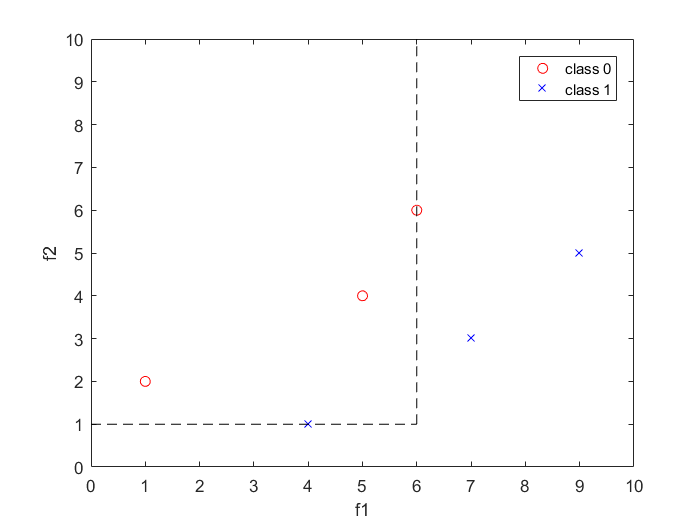
\includegraphics[scale=0.4]{coordinate1.png}  
 	\caption{划分规则} 
 	\label{coordinate1}
 \end{figure}
 \item [(3)]
 规则如图2所示。按照$f_2\leq 2$来划分,将$D$分成了$D^1$和$D^2$两个部分。其中$D^1$包含第一个和第四个样例。由此可得
 \begin{equation}
 Ent(D^1) =  -(\frac{1}{2}\log_2\frac{1}{2} + \frac{1}{2}\log_2\frac{1}{2}) = 1.000
 \end{equation}
 \begin{equation}
 Ent(D^2) = -(\frac{2}{4}\log_2\frac{2}{4} + \frac{2}{4}\log_2\frac{2}{4}) = 1.000
 \end{equation}
 所以可得信息增益为
 \begin{equation}
 \begin{aligned}
 Gain(D, f_2\leq 2) &= Ent(D) - \sum_{v=1}^{2}\frac{|D^v|}{|D|}Ent(D^v)\\
 &= 1 - (\frac{2}{6}\times 1 + \frac{4}{6}\times 1)\\
 &= 0
 \end{aligned}
 \end{equation}
 \begin{figure}[!h]
 	\centering   
 	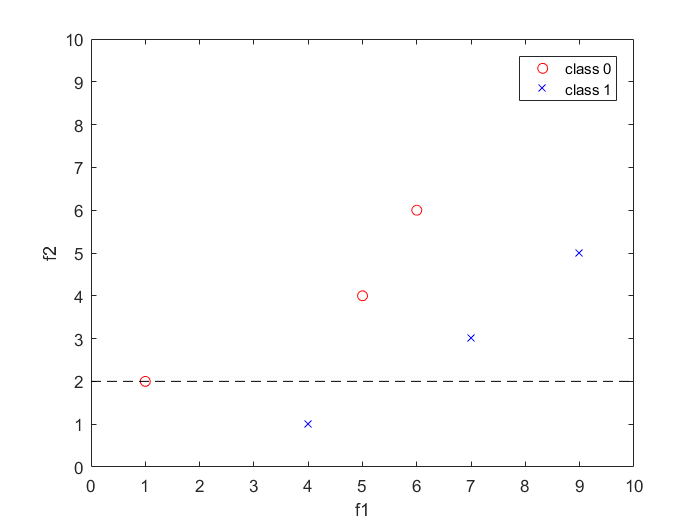
\includegraphics[scale=0.4]{coordinate2.png}  
 	\caption{划分规则} 
 	\label{coordinate2}
 \end{figure}
 \end{enumerate}
 \end{solution}
\newpage

\section{[25pts] Universal Approximator}
已知函数$f:[-1, 1]^n \mapsto [-1, 1]$满足$\rho$-Lipschitz性质。 给定误差$\epsilon > 0$,请构造一个激活函数为\mbox{ sgn($\mathbf{x}$) }的神经网络$ \mathcal{N}:[-1,1]^n \mapsto [-1,1] $,使得对于任意的输入样本$ \mathbf{x} \in [-1,1]^n $,有$|f(\mathbf{x}) - \mathcal{N}(\mathbf{x})| \leq \epsilon$。\\
(Lipschitz条件参见\href{https://en.wikipedia.org/wiki/Lipschitz_continuity}{Wikipedia},其中\mbox{ sgn($\mathbf{x}$) }的定义参见《机器学习》第98页。)

\begin{enumerate}[ {(}1{)}]
	\item \textbf{[5pts]} 请画出构造的神经网络$\mathcal{N}$的示意图;
	
	\item \textbf{[10pts]} 请对构造的神经网络进行简要的说明(写清每一层的线性组合形式,也就是结点间的连接方式和对应的权重);
	
	\item \textbf{[10pts]} 证明自己构造的神经网络的拟合误差满足要求。
\end{enumerate}


\begin{solution}

\begin{enumerate}[ {(}1{)}]
\item 神经网络$\mathcal{N}$的示意图如下所示(因为空间有限,所以省略了部分结点和边,以及所有权值为0的边均在图中省略):
\begin{figure}[!h]
	\centering   
	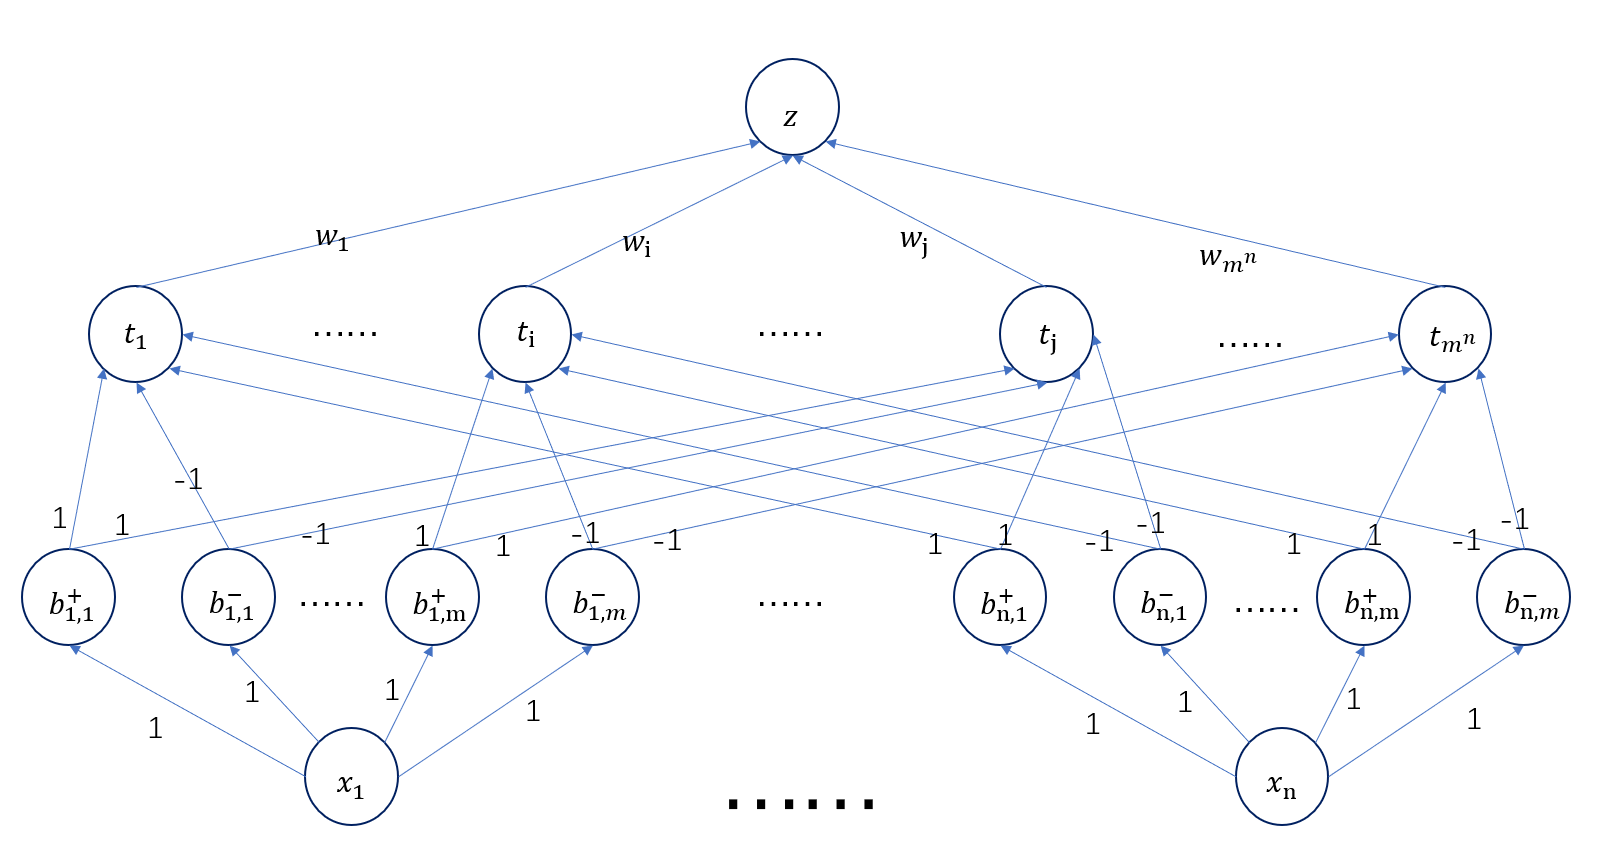
\includegraphics[scale=0.5]{net.png}  
	\caption{神经网络$\mathcal{N}$} 
	\label{net}
\end{figure}\\
如上图所示,输入层$n$个神经元$x_1,...,x_n$,从输入层到第一个隐层,$x_i$只和$b_{i,j}^+$以及$b_{i,j}^-$相连,权重为$1$。第一个隐层共有$2nm$个神经元$b_{1,1}^+,b_{1,1}^-,...,b_{n,m}^+,b_{n,m}^-$,阈值暂时没有画在图中,将在之后解释,$b_{i,j}^+$连接特定的$t_s$,权重为$1$,$b_{i,j}^-$连接特定的$t_s$,权重为$-1$。第二个隐层的阈值暂时没有画在图中,将在之后解释,所有的$t_s$都连接到输出神经元,权值为$w_s$。(以上说明中,关于“连接到”,也可以理解为没有连接到的点之间权值为0)\\
	
\item 
\textbf{$\mathcal{N}$的结构:}\\
神经网络分为$4$层,其中包括输入层,输出层和两个隐层。其中输入层有$n$个输入单元(每个单元对应了一个$\mathbf{x}$的维度的数值),第一个隐层(以后称为B层)有$2mn$个单元,第二个隐层(以后称为T层)有$m^n$个单元,输出层只有一个单元也就是整个神经网络的输出值。\\
\textbf{$\mathcal{N}$的符号表示:}
见下表:
\begin{table}[!h]
	\centering
	\caption{符号表}
	\label{my-label}
	\begin{tabular}{|l|l|}
		\hline
	\textbf{符号}	& \textbf{描述} \\ \hline
	$x_i$	& 输入单元接受的输入值,也就是$ \mathbf{x} $向量的各个维度的数值 \\ \hline
	$b_{i,j}^+, b_{i,j}^-$	& B层的单元,注意到$b_{i,j}^+$和$b_{i,j}^-$是成对出现的 \\ \hline
	$\alpha_{i,j}^+,\alpha_{i,j}^-$	& 分别是$b_{i,j}^+$和$b_{i,j}^-$的输入 \\ \hline
	$\beta_{i,j}^+,\beta_{i,j}^-$	& 分别是$b_{i,j}^+$和$b_{i,j}^-$的输出 \\ \hline
	$\theta_{i,j}^+,\theta_{i,j}^-$	& 分别是$b_{i,j}^+$和$b_{i,j}^-$的阈值 \\ \hline
	$t_i$	& T层的单元 \\ \hline
	$\gamma_i$	& $t_i$的输入 \\ \hline
	$\delta_i$	& $t_i$的输出 \\ \hline
	$\lambda_i$	& $t_i$的阈值 \\ \hline
	$z$	& 输出层的单元的输出值 \\ \hline
	$\rho$	& 函数$f$的Lipschitz常数 \\ \hline
	$m$	& 神经网络的超参数,用于控制B层的神经元的数目\\ \hline
	$\sigma$	& $\sigma>0$,加在$\theta_{i,m}^-$上,确保$x_i=1$时也能正确处理\\ \hline
	\end{tabular}
\end{table}\\
\textbf{$\mathcal{N}$的各层的线性组合形式:}\\
输入层神经元数目:$n$,即$x_1, x_2,...,x_n$\\
B层神经元数目:$2mn$,即$b_{1,1}^*,...,b_{1,m}^*,...,b_{n,1}^*,...,b_{n,m}^*\ ,\ \ *\in \{+,-\}$\\
T层神经元数目:$m^n$,即$t_1,t_2,...,t_{m^n}$\\
输出层神经元数目:$1$,即$z$\\
从输入层到B层的传播:
\begin{equation}
\alpha_{i,j}^* = x_i\ ,\ \ *\in \{+,-\}
\end{equation}
B层的神经元计算:
\begin{equation}
\theta_{i,j}^+ = -1 + (j-1)\frac{2}{m}\\
\end{equation}
\begin{equation}
\theta_{i,j}^- =
\begin{cases}
-1 + j\frac{2}{m} & 1\leq j\leq m-1;\\
-1 + j\frac{2}{m} + \sigma = 1 + \sigma & j = m;
\end{cases}
\end{equation}
\begin{equation}
\beta_{i,j}^* = sgn(\alpha_{i,j}^* - \theta_{i,j}^*)\ ,\ \ *\in \{+, -\}
\end{equation}
从B层到T层,映射较为复杂:B层的神经元$b_{1, index_1}^+,b_{2,index_2}^+,...,b_{n,index_n}^+$的输出乘以权重$1$以及$b_{1, index_1}^-,b_{2,index_2}^-,...,b_{n,index_n}^-$的输出乘以权重$-1$之后作为$t_s$的输入值,其中$s= 1+\sum_{i=1}^{n}(index_i-1)m^{(i-1)} $,所以为了根据$s$得到$index_i$,给出以下算法:
\begin{algorithm}[h]  
	\caption{IndexTranslate}  
	\begin{algorithmic}[1]  
		\Require  
		$s$ : T层的神经元编号 
		\Ensure  
		$(index_1,index_2,...,index_n)$ : 输入到$t_s$的B层神经元的编号
		\State $s = s-1$ 
		\For{i from 1 to n}  
		\State $index_i = s \mod m^i$
		\State $s = s - index_i$
		\State $index_i = index_i + 1$
		\EndFor
		\label{code:recentEnd}  
	\end{algorithmic}  
\end{algorithm}\\
现在给出从B层到T层的传播:
\begin{equation}
(index_1, index_2,...,index_n) = IndexTranslate(s)
\end{equation}
\begin{equation}
\gamma_s = \sum_{i=1}^{n}\beta_{i,index_i}^+ - \sum_{i=1}^{n}\beta_{i,index_i}^-
\end{equation}
T层的神经元计算:\\
\begin{equation}
\lambda_s = n - \frac{1}{2}
\end{equation}
\begin{equation}
\delta_s = sgn(\gamma_s - \lambda_s)
\end{equation}
从T层到输出层的边的权值其实是函数$f$在某些点的值,下面给出算法通过$t_s$的编号$s$来计算$\delta_s$对应的权值:
\begin{algorithm}[h]  
	\caption{GetWeightFromIndex}  
	\begin{algorithmic}[1]  
		\Require  
		$s$ : T层的神经元编号  
		\Ensure  
		$w_s$ : 从T层到输出层的边中$\delta_s$对应的边的权重
		\State $(index_1, index_2,...,index_n) = IndexTranslate(s)$ 
		\For{i from 1 to n}  
		\State $xt_i = -1 + (index_i - \frac{1}{2})\frac{2}{m}$
		\EndFor
		\State $\mathbf{xt} = [xt_1, xt_2,...,xt_n] $
		\State $w_s = f(\mathbf{xt})$
		\label{code:recentEnd}  
	\end{algorithmic}  
\end{algorithm}\\
通过上述算法计算每一个$\delta_i$的权值$w_i = GetWeightFromIndex(i)$。\\
输出层的最终输出:
\begin{equation}
z = \sum_{i=1}^{m^n}w_i\delta_i
\end{equation}
\item 证明:\\
在进行具体的证明之前,首先对神经网络$\mathcal{N}$的设计思路进行说明:由于需要逼近的函数$f$具有Lipschitz性质,即:
\begin{equation}
|f(\mathbf{x}) - f(\mathbf{y})| \leq \rho||\mathbf{x} - \mathbf{y}||
\end{equation}
所以$\mathcal{N}$的大致思想就是将$f$的定义域分割成很多个足够小的子空间,根据Lipschitz性质,子空间内的任意两个点$\mathbf{x}$和$\mathbf{y}$对应的函数值$f(\mathbf{x})$和$f(\mathbf{y})$相差会有一个上界即$\rho||\mathbf{x} - \mathbf{y}||$。只要确定了分割的子空间的大小,那么$||\mathbf{x} - \mathbf{y}||$也会随之确定。所以只要确保将定义域分割的足够细使得$\rho||\mathbf{x} - \mathbf{y}|| \leq \epsilon$即可得到符合题意的神经网络。考虑到有限维向量范数的等价性,为了方便之后的证明,在这里取2-范数(即便取其他范数,我们的结论仍然不会改变,这个将在之后证明),即:
\begin{equation}
|f(\mathbf{x}) - f(\mathbf{y})| \leq \rho||\mathbf{x} - \mathbf{y}||_2
\end{equation}
证明之前先设置神经网络超参数:
\begin{equation}
m=\left\lceil\frac{\rho\sqrt{n}}{\epsilon}\right\rceil	
\end{equation}
然后将定义域空间$[-1,1]^n$等分成$m^n$份,具体的:对于维度$i$,将其等分为$m$份,得到$m$个区间$[-1, -1+\frac{2}{m}),\ [-1+\frac{2}{m},-1+2\frac{2}{m}),\ ...,\ [-1 + (m-1)\frac{2}{m}, 1]$,每个区间的长度为$\frac{2}{m}$(注意到最后一个区间两边都是闭的)。现在定义$D_{i,j}$表示第$i$维的第$j$个区间即$D_{i,j} = [-1+(j-1)\frac{2}{m},-1+j\frac{2}{m})$,在此基础上再定义子空间$S(j_1,j_2,...,j_n) = D_{1,j_1} \times D_{2,j_2} \times ... \times D_{n, j_n}$。\\
下证:对于对于任意的输入样本$ \mathbf{x} \in [-1,1]^n $,有$|f(\mathbf{x}) - \mathcal{N}(\mathbf{x})| \leq \epsilon$。\\\\
\textbf{case 1:}\\
$ \mathbf{x} \in [-1,1)^n $\\
考虑$\mathbf{x}$的每一个维度的值$(x_1,...,x_n)$,不失一般性的假设$\mathbf{x} \in S(index_1, index_2,..,index_n)$,即:
\begin{equation}
\begin{aligned}
x_1 \in [-1+(index_1 &- 1)\frac{2}{m},-1 + index_1\frac{2}{m}) \\
x_2 \in [-1+(index_2 &- 1)\frac{2}{m},-1 + index_2\frac{2}{m}) \\
&......\\
x_n \in [-1+(index_n &- 1)\frac{2}{m},-1 + index_n\frac{2}{m})
\end{aligned}
\end{equation}
现在观察到任意$i$,都有$x_i \geq -1+(index_i - 1)\frac{2}{m}$以及$x_i < -1+index_i\frac{2}{m}$,结合$(3.3)$可得:
\begin{equation}
\begin{aligned}
&\beta_{i,j}^* = 1\ \ \ for\ *\in \{+,-\}\ and\ j < index_i\\
&\beta_{i,index_i}^+ = 1\\
&\beta_{i,index_i}^- = 0\\
&\beta_{i,j}^* = 0\ \ \ for\ *\in \{+,-\}\ and\ j > index_i
\end{aligned}
\end{equation}
现在定义$s= 1+\sum_{i=1}^{n}(index_i-1)m^{(i-1)}$,又根据$(3.6)$可得:
\begin{equation}
\gamma_s = \sum_{i=1}^{n}\beta_{i,index_i}^+ - \sum_{i=1}^{n}\beta_{i,index_i}^- = n
\end{equation}
现在再考虑$s'$且$s'\neq s$,定义$(index_1', index_2',...,index_n') = IndexTranslate(s')$,由于$s'\neq s$,所以一定存在$i$使得$index_i\neq index_i'$,那么根据$(3.13)$可得$\beta_{i,index_i'}^+ - \beta_{i,index_i'}^- = 0$,即:
\begin{equation}
\gamma_{s'} \leq n-1,\ \ \ for\ s'\neq s
\end{equation}
又因为$\lambda_s = \lambda_{s'} = n - \frac{1}{2}$,所以根据$(3.8)$可得:
\begin{equation}
\begin{aligned}
&\delta_s = sgn(\gamma_s - \lambda_s) = 1\\
&\delta_{s'} = sgn(\gamma_{s'} - \lambda_{s'}) = 0\ \ \ for\ s'\neq s
\end{aligned}
\end{equation}
结合上式再根据$(3.9)$可得:
\begin{equation}
z = \sum_{i=1}^{m^n}w_i\delta_i = w_s\delta_s = GetWeightFromIndex(s)
\end{equation}
根据$Algorithm\ 2$可知$GetWeightFromIndex(s) = w_s = f(\mathbf{xt})$其中$\mathbf{xt} = [xt_1,...xt_n]$而且$xt_i=-1 + (index_i - \frac{1}{2})\frac{2}{m}$,所以神经网络最终的输出就是$\mathcal{N}(x) = f(\mathbf{xt})$,现在证明$|f(\mathbf{x})-f(\mathbf{xt})| < \epsilon$。\\
因为$x_i \in [-1+(index_i - 1)\frac{2}{m},-1 + index_i\frac{2}{m})$且$xt_i=-1 + (index_i - \frac{1}{2})\frac{2}{m}$,所以$|x_i - xt_i|\leq \frac{1}{m}$,所以可得:
\begin{equation}
||\mathbf{x} - \mathbf{xt}||_2 = \sqrt{|x_1 - xt_1|^2 + ...+|x_n-xt_n|^2} \leq \frac{\sqrt{n}}{m}
\end{equation}
所以根据Lipschitz性质,有:
\begin{equation}
|f(\mathbf{x}) - f(\mathbf{xt})| \leq \rho||\mathbf{x} - \mathbf{xt}||_2  \leq \rho\frac{\sqrt{n}}{m}
\end{equation}
再根据超参数$m=\left\lceil\frac{\rho\sqrt{n}}{\epsilon}\right\rceil$可得:
\begin{equation}
|f(\mathbf{x}) - f(\mathbf{xt})| \leq \rho\frac{\sqrt{n}}{m} \leq \rho\frac{\sqrt{n}\epsilon}{\rho\sqrt{n}} = \epsilon
\end{equation}
又因为$\mathcal{N}(x) = f(\mathbf{xt})$,所以:
\begin{equation}
|f(\mathbf{x}) - \mathcal{N}(\mathbf{x})| \leq \epsilon
\end{equation}
由此得证。\\\\
\textbf{case 2:}\\
$\mathbf{x} = (1,1,...,1)$\\
根据$(3.3)$可得$\theta_{i,m}^- = 1+\sigma > 1$,所以有:
\begin{equation}
\begin{aligned}
&\beta_{i,j}^* = 1\ \ \ for\ *\in \{+,-\}\ and\ j < m\\
&\beta_{i,m}^+ = 1\\
&\beta_{i,m}^- = 0\\
\end{aligned}
\end{equation}
相应的,有:
\begin{equation}
\begin{aligned}
&\delta_i = 0\ \ \ for\ i < m^n\\
&\delta_{m^n} = 1
\end{aligned}
\end{equation}
故$\mathcal{N}(\mathbf{x}) = f(\mathbf{xt})$且$xt_i = 1 - \frac{1}{m}$,通过\textbf{case 1}的证明易得$|f(\mathbf{x}) - \mathcal{N}(\mathbf{x})| \leq \epsilon$。\\\\
现在考虑$||\mathbf{x}-\mathbf{xt}||$不取2-范数的情况,因为有限维范数的等价性,所以对于p-范数,有:
\begin{equation}
C_1||\mathbf{x}-\mathbf{xt}||_2 \leq ||\mathbf{x}-\mathbf{xt}||_p \leq C_2||\mathbf{x}-\mathbf{xt}||_2
\end{equation}
所以$|f(\mathbf{x}) - f(\mathbf{xt})| \leq \rho||\mathbf{x} - \mathbf{xt}||_p  \leq C_2\rho\frac{\sqrt{n}}{m}$,只要设置超参数$m=\left\lceil\frac{\rho\sqrt{n}}{C_2\epsilon}\right\rceil$就可以得到相同的结论。\\
综上所述,可得对于任意的输入样本$ \mathbf{x} \in [-1,1]^n $,有$|f(\mathbf{x}) - \mathcal{N}(\mathbf{x})| \leq \epsilon$。
\end{enumerate}


\end{solution}
\newpage

\section{[40pts] Neural Network in Practice}
通过《机器学习》课本第5章的学习,相信大家已经对神经网络有了初步的理解。深度神经网络在某些现实机器学习问题,如图像、自然语言处理等表现优异。本次作业旨在引导大家学习使用一种深度神经网络工具,快速搭建、训练深度神经网络,完成分类任务。

我们选取PyTorch为本次实验的深度神经网络工具,有了基础工具,我们就能如同搭积木一样构建深度神经网络。\href{http://pytorch.org/}{PyTorch}是Facebook开发的一种开源深度学习框架,有安装方便、文档齐全、构架方便、训练效率高等特点。本次作业的首要任务就是安装PyTorch。

目前PyTorch仅支持Linux和MacOS操作系统,所以Window用户需要装一个Linux虚拟机或者直接安装Linux系统。PyTorch安装很方便,只需要在其主页中的Get Start一栏选择对应的环境设置,便能够一键安装。有GPU的同学也可以尝试安装GPU版本的PyTorch。为保证此次作业的公平性,只要求使用CPU进行网络训练,当然有条件的同学也可以尝试使用GPU进行训练。在批改作业时,助教会提供Python 2.7、3.5、3.6三种环境进行实验验证。

我们选取CIFAR10作为本次作业的训练任务。\href{https://en.wikipedia.org/wiki/CIFAR-10}{CIFAR10}是一个经典的图片分类数据集,数据集中总共有60000张32$\times$32的彩色图片,总共有10类,每类6000张图片,其中50000张图片构成训练集,10000张图片构成测试集。PyTorch通过torchvision给用户提供了获取CIFAR10的方法,详细信息可见\href{http://pytorch.org/tutorials/beginner/blitz/cifar10_tutorial.html}{PyTorch的教程}。此外关于CIFAR10分类准确率排行可见此\href{http://rodrigob.github.io/are_we_there_yet/build/classification_datasets_results.html}{链接}。

下面我们将尝试使用PyTorch来解决实际问题:

\begin{enumerate}[(1)]
	\item \textbf{[15pts]} 首先我们跟随PyTorch的教程,用一个简单的卷积神经网络(Convolutional Neural Network, CNN),完成CIFAR10上的分类任务,具体要求如下:
	
	\begin{itemize}
		\item \textbf{[7pts]} 在代码实现之前,大家可能需要对CNN网络进行一定的了解,请大家自行查阅资料(PyTorch的教程中也有部分介绍CNN网络),并在实验报告中给出对CNN的见解:主要回答什么是卷积层,什么是Pooling层,以及两者的作用分别是什么;
		\item \textbf{[8pts]} 接下来就是具体的代码实现和训练。教程会手把手教你完成一次训练过程,其中使用SGD作为优化方法,请同学们自行调整epoch的大小和学习率,完成此次训练。另外,请在实验报告中给出必要的参数设置,以及训练结果如最终的loss、在测试集上的准确率等;
	\end{itemize}
	\item \textbf{[20pts]} 显然,这样一个简单的网络在CIFAR10上并不能取得令人满意的结果,我们需要选取一个更为复杂的网络来提升训练效果。在此小题中,我们选取了CIFAR10准确率排行榜上排名第二的结构,具体参见\href{https://arxiv.org/pdf/1412.6806.pdf}{论文链接}。为了方便大家实现,我们直接给出了网络结构如图\ref{network_structure}所示。请大家搭建完成此网络结构,并选择Adam为优化器,自行调整相关参数完成训练和预测,实验结果报告内容同第(1)小题;
	\begin{figure}[!h]
		\centering   
		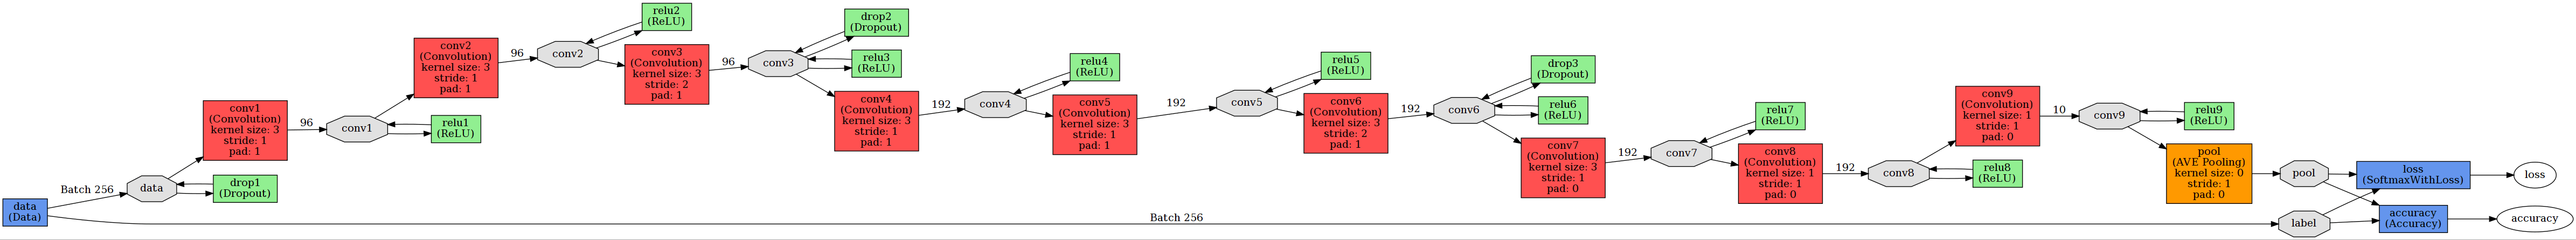
\includegraphics[width=0.99\textwidth, height=0.15\textwidth]{nn_structure.png}  
		\caption{待实现网络结构} 
		\label{network_structure}
	\end{figure}
	\item \textbf{[5pts]} 通过上一题实验我们可以发现,即使使用现成的网络结构也不一定能达到与其相同的训练效果。请大家分析其中的原因,并谈谈本次实验的感想,以及对深度学习调参的体会。
\end{enumerate}

\noindent{\textbf{实验报告.}}

\begin{enumerate}
\item [(1)]
\textbf{对CNN的见解}:卷积神经网络是一种非常强大的,适合用于图像,视频识别以及自然语言处理的神经网络的。卷积神经网络本身就是一种特殊的神经网络,其训练的流程为:输入层接受训练集数据,通过隐层一层层传递到输出层,输出与真实标签进行比较,得到损失函数,然后再通过反向传播来调整隐层的参数,进而降低损失函数,来使得预测结果逼近与真实标签。CNN中比较特殊的隐层结构是卷积层和pooling层,其中卷积层主要承担了对特定模式的识别工作,pooling层主要起到了采样的作用。\\\\
\textbf{卷积层的概念}:是卷积神经网络的核心,承担了卷积神经网络大部分的工作量。\\\\
\textbf{卷积层的作用}:卷积层的作用主要在于提取特征,这个操作类似于信号处理中的滤波,和人类大脑认知世界也有几分相似。这个操作的实现用到了卷积的方法。具体的,如果输入的数据大小为$H\times W\times D$(此处先假设batch size为1,其中D表示channel数量),那么卷积层就会有诸多大小为$H'\times W'\times D$的filter(其中$H' < H$而且$W' < W$)。通过将一个filter“覆盖”在输入数据上,会得到输入数据上的一个和filter相同大小的数据块,把数据块和filter对应位置的元素相乘然后求和,可以得到一个标量值,把filter“覆盖”到数据的不同位置可以得到很多标量值,将这些标量值按照顺序排列起来可以得到一个activation map,每一个filter针对每一个输入数据都会得到一个activation map,然后把多个filter对应的activation map堆叠在一起就可以得到下一个隐层的输入数据。每一个卷积层得到的activation map其实就是对某种特征的提取,如果map中某个元素值很大,就说明这个元素对应的输入数据的特定位置有可能存在某种特征。所以activation map实际上可以反应出特征在输入数据集中的分布。卷积层可以识别的特征多种多样的,一般第一卷积层只能识别一些简单的特征,例如边缘,曲线,角,更多层的卷积层可以识别到更加复杂的特征。\\\\
\textbf{Pooling层的概念}:pooling层也是卷积神经网络中一个重要的结构,他的主要功能在于对数据进行采样。\\\\
\textbf{Pooling层的作用}:总体来讲pooling层的作用在于减少数据大小,减少参数,降低运算量,减低训练时间,防止过拟合,提高泛化能力,同时还可以保持特征的不变形(包括平移,旋转,尺度等方面)。具体的,pooling层就是按照一定的比例对输入数据进行采样,常见的有max-pooling和average-pooling。常见的做法是将数据分成$2\times 2$的数据块然后从每个数据块中选择一个最大值(或者平均值)来代替整个数据块。其中max-pooling采样操作还能够保持输入数据的特征不变型,比如说某个数据块中出现了某个特征,反映在输入数据上就是某个元素的值非常大。当我们在对这个数据块采样的时候,为了在下一层维持这个特征的表现,我们选择了最大的数值作为采样后的结果,这背后蕴含了即便数据缩小了,我们仍然尽可能保持原有的特征这一思想,所以实践中往往max-pooling表现会比较好。实践中会在卷积层之间周期性的插入pooling层来提升整体的效果。\\
\textbf{官方教程CNN实验过程:}在pytorch官网下载对应版本之后,跟着教程训练了一个简单的卷积神经网络,其中包括卷积层,pooling层,全连接层,最终得到实验结果。\\
\textbf{模型结构:}
\begin{figure}[!h]
	\centering   
	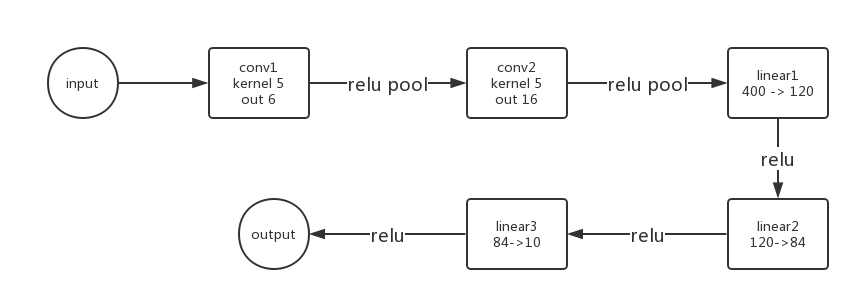
\includegraphics[scale=0.5]{ng1.png}  
	\caption{简单CNN} 
	\label{ng1}
\end{figure}\\
\textbf{官方教程CNN实验的参数设置如下:}
\begin{table}[h]
	\centering
	\caption{官方教程CNN参数设置}
	\label{cn1}
	\begin{tabular}{|l|l|l|l|l|}
		\hline
		参数	& batch size & epoch & learning rate & momentum \\ \hline
		设定值	& 4 & 40 & 0.0005 & 0.9 \\ \hline
	\end{tabular}
\end{table}\\
选择epoch为40是考虑到模型在40个epoch之后loss就很难下降而且出现了明显的震荡,选择learning rate为0.0005是因为如果把rate调大,SGD效果反而变差,如果把rate调小,那么SGD下降会变慢,训练结果对比见下图(下图中横坐标表示训练的张次数,即1张图片训练1次为1张次数):
\begin{figure}[htbp]
	\centering
	\begin{minipage}[t]{0.48\textwidth}
		\centering
		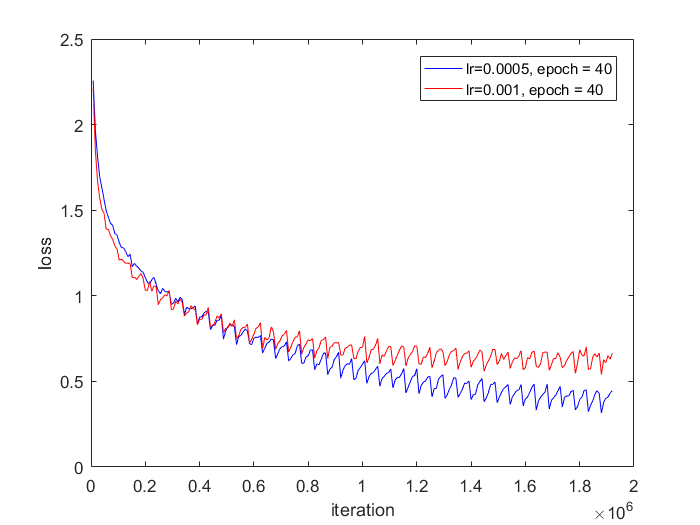
\includegraphics[width=6cm]{net-0005-001-40.png}
		\caption{epoch=40, rate=0.0005 or 0.001}
	\end{minipage}
	\begin{minipage}[t]{0.48\textwidth}
		\centering
		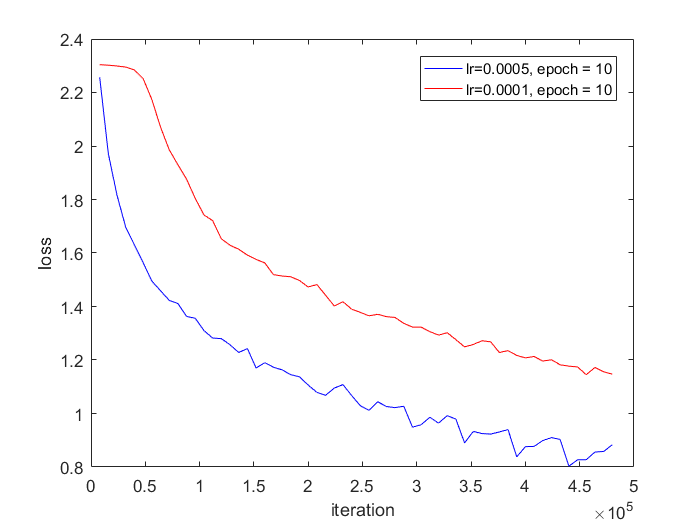
\includegraphics[width=6cm]{net-0005-0001-10.png}
		\caption{epoch=10, rate=0.0005 or 0.0001}
	\end{minipage}
\end{figure}\\
设置epoch=40,对比rate=0.0005和rate=0.001的模型的训练效果,发现随着迭代次数增加前者下降的更快。\\
设置epoch=10,对比rate=0.0005和rate=0.0001的模型的训练效果,发现前者下降明显快于后者。\\
最终通过对比实验确定模型的参数如上。\\
\textbf{训练结果:}\\
\textbf{最终loss:}采用的计算loss的方式为cross entropy loss,\textbf{最终loss的大小为:$0.664$}。\\
\textbf{测试集上的准确率:}
\begin{table}[h]
	\centering
	\caption{简单CNN准确率}
	\label{ac2}
	\begin{tabular}{|l|l|l|l|l|l|l|l|l|l|l|l|}
		\hline
	类别	& plane & car & bird & cat & deer & dog & frog & horse & ship & truck & total \\ \hline
	准确率	& 0.67 & 0.73 & 0.46 & 0.43 & 0.48 & 0.43 & 0.68 & 0.63 & 0.70 & 0.68 & 0.59 \\ \hline
	\end{tabular}
\end{table}\\
综合准确率为$0.59$。\\
\textbf{实验小结:}
本次实验的模型只是tutorial中给出的简单模型,结构不复杂,训练时间开销也不大。但是调整参数,选择参数的过程也不容忽视,如何高效锁定最优的参数的范围是个值得探究的问题,二分法有时候也可以应用在这种场景中,可以提高调参的效率。
\item [(2)]
\textbf{ALL-CONV-NET实验过程:}仿照上一个简单CNN的实验,实现ALL-CONV-NET的结构并进行测试。在实验过程中,发现给定的网络结构十分复杂,训练时间开销巨大,准确率提升缓慢,所以决定修改简化模型,调整参数,最终实现了简化后的ALL-CONV-NET-S模型。由于机器性能有限,作业时间有限以及自己掌握的深度学习知识有限,所以并没有能够复现出论文中的高准确率,但是相比于简单CNN模型,已经有了巨大的提升,同时时间开销也是可以忍受的。\\
\textbf{修改简化模型:}\\
简化后结构如下图所示:
\begin{figure}[!h]
	\centering   
	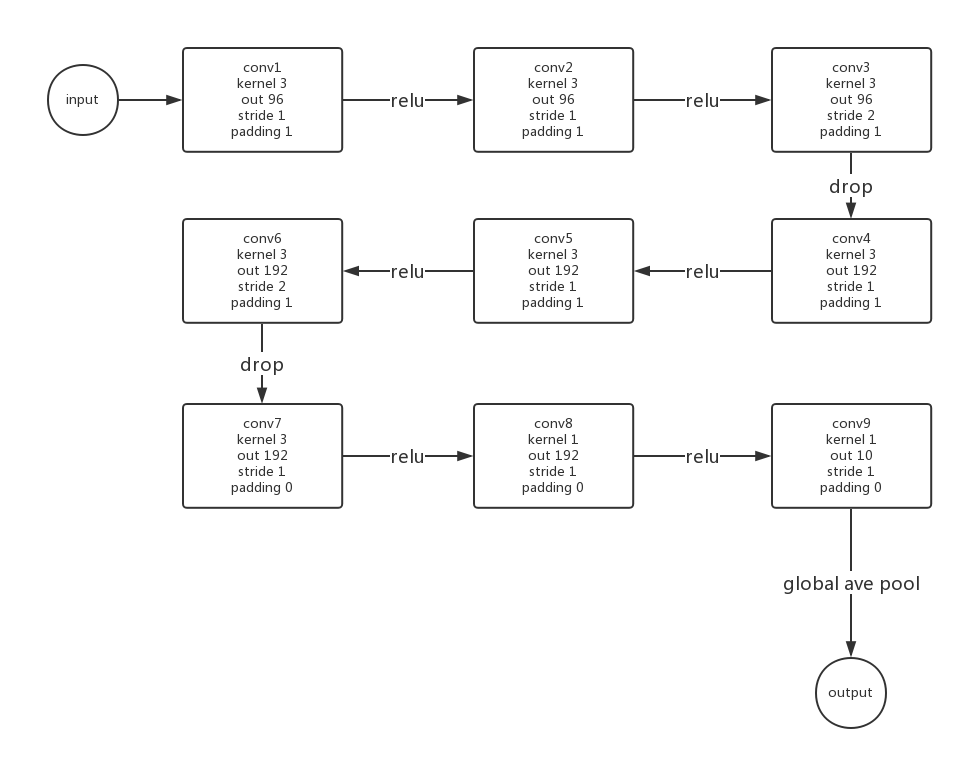
\includegraphics[scale=0.3]{ng2.png}  
	\caption{ALL-CONV-NET-S} 
	\label{ng2}
\end{figure}\\
简化的模型删去了3个relu层和1个dropout层。
改进后的模型在降低了复杂度的同时,提高了训练效率,降低了时间开销,具体对比如下:
\begin{figure}[!h]
	\centering   
	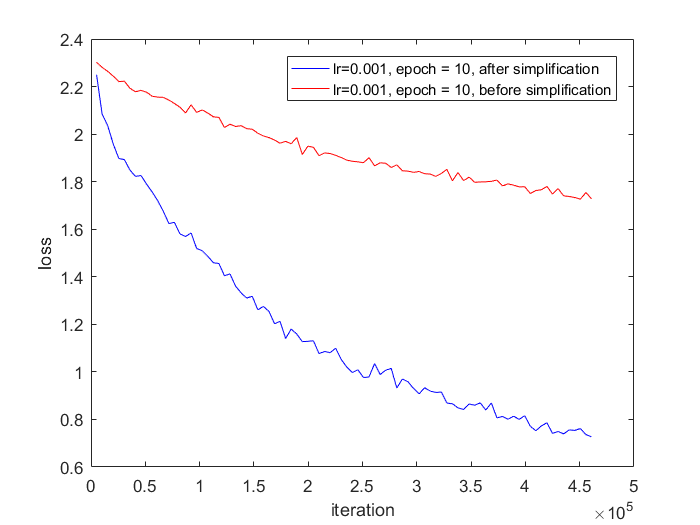
\includegraphics[scale=0.5]{after-before-simplification.png}  
	\caption{ALL-CONV-NET简化前后对比} 
	\label{acn0}
\end{figure}\\
\textbf{参数设置如下:}
\begin{table}[h]
	\centering
	\caption{ALL-CONV-NET-S参数设置}
	\label{acn1}
	\begin{tabular}{|l|l|l|l|}
		\hline
	参数	& batch size & epoch & learning rate \\ \hline
	设定值	& 256 & 40 & 0.001 \\ \hline
	\end{tabular}
\end{table}\\
选择epoch为40是因为模型在40个epoch的训练之后loss的下降就十分缓慢了,而且准确率的提升也十分缓慢,甚至50个epoch之后仍然和40个epoch的准确率一样,同时考虑到时间开销,机器负载,所以在40个epoch之后就停止训练。选择learning rate为0.001也是比较出来的结果,如果调大,那么随着轮数增大,效果会变差,如果太小,那么训练的效率也会变得低下。训练结果对比如下图所示(下图中横坐标表示训练的张次数,即1张图片训练1次为1张次数):
\begin{figure}[htbp]
	\centering
	\begin{minipage}[t]{0.48\textwidth}
		\centering
		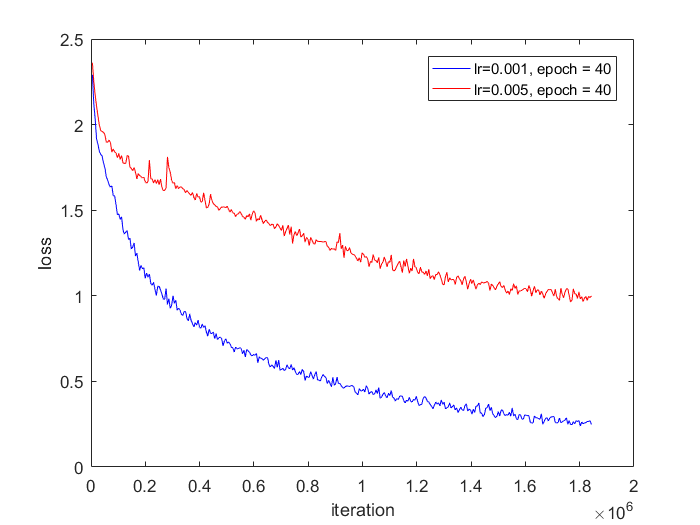
\includegraphics[width=6cm]{acns-001-005-40.png}
		\caption{epoch=40, rate=0.001 or 0.005}
	\end{minipage}
	\begin{minipage}[t]{0.48\textwidth}
		\centering
		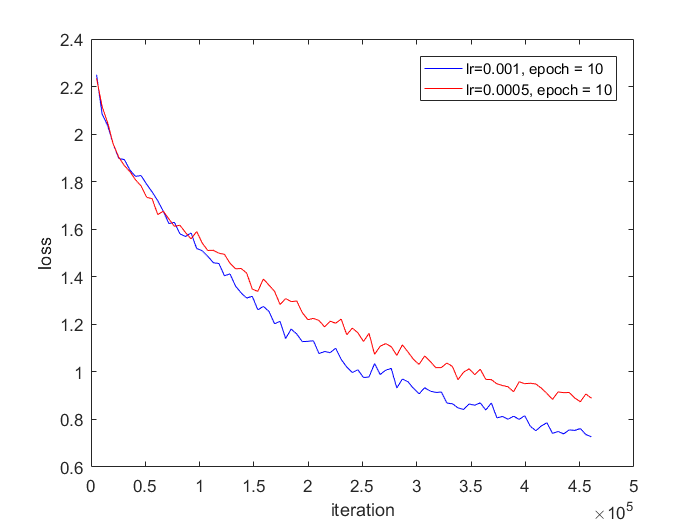
\includegraphics[width=6cm]{acns-001-0005-10.png}
		\caption{epoch=10, rate=0.001 or 0.0005}
	\end{minipage}
\end{figure}\\
设置epoch=40,对比rate=0.001和rate=0.005的模型的训练效果,发现明显前者下降的更快。\\
设置epoch=10,对比rate=0.001和rate=0.0005的模型的训练效果,发现前者下降快于后者。\\
最终通过对比实验确定模型的参数如上。\\
\textbf{训练结果:}\\
\textbf{最终loss:}采用的计算loss的方式为cross entropy loss,\textbf{最终loss的大小为:$0.248$}。\\
\textbf{测试集上的准确率:}
\begin{table}[h]
	\centering
	\caption{简单CNN准确率}
	\label{ac1}
	\begin{tabular}{|l|l|l|l|l|l|l|l|l|l|l|l|}
		\hline
		类别	& plane & car & bird & cat & deer & dog & frog & horse & ship & truck & total \\ \hline
		准确率	& 0.75 & 1.00 & 0.92 & 0.68 & 0.76 & 0.60 & 0.72 & 0.91 & 0.90 & 0.94 & 0.80 \\ \hline
	\end{tabular}
\end{table}\\
综合准确率为$0.80$。\\
\textbf{实验小结:}
ALL-CONV-NET-S的模型比起之前的模型结构复杂很多,训练过程也复杂很多,时间开销也很大,如果不用GPU来跑恐怕很难进行实验。实验过程中遇到这些问题:\\
训练时间太长,而且效果不满意,甚至效率远不如简单模型 -- 这通过调整参数,尤其是学习率,以及简化模型来解决。模型简化后不仅训练时间降低,而且效果也有上升,但是相应的,从长远来看,简化的模型还是不如原来的模型。\\
很难确定训练的epoch,有时候epoch过大之后,后期的训练几乎没有什么明显效果 -- 这个是通过绘制epoch次数和loss的图像来判断分析,通过观察折现的走势,可以得到在什么时候终止实验可以平衡时间开销和准确率亮点,即,时间开销可以忍受同时准确率也较高。\\
出现了过拟合 -- 这个可以用pooling和dropout来解决,同时也可以减低训练时间\\

\item [(3)]
\textbf{分析原因:}第二个实验使用了CIFAR10准确率排行榜上第二的结构进行实验,然而事实上自己训练出的效果明显不如论文中给出的结论,仅仅有$0.8$的综合准确率,探究原因应该是多方面的。\\
首先复现论文的内容本身就是不容易的工作,需要一定的经验积累,对于第一次编写CNN程序,确实会因为经验不足走很多弯路。\\
考虑到自己使用的模型是原来的模型进行了一些修改简化,所以虽然在短期训练中得到了不错的结果,但是长远来看效果不如论文中给出的模型。\\
虽然使用的模型是一样的,但是复现过程不仅仅是搭建模型,还有训练本身,在pytorch中使用的优化算法为Adam,采用的是默认参数,但是这未必是论文作者使用的优化配置,而且论文作者使用的框架也未必是pytorch,不同框架对于同一种优化算法的实现虽然基本是一致的,但是实现细节上可能也会有所不同,采用的默认参数设置也会有不同,这都可能导致不同的结果。\\
由于本次实验是作业的一部分,而同时还有其他课业任务,以及作业的DDL的客观存在,所以在实验训练模型时无法像模型提出者一样使用先进的设备全心全力的进行模型的训练调整(与此对比,作为学生的我们只有自己的家用电脑,有些同学甚至没有N卡,当然也有同学选择租赁云服务器)。\\
综上所述,无法完全复现出论文的结果,既有自身能力不足的主观原因,又有一些不可避免的客观原因。\\
\textbf{实验感想:}本次实验包含对两个CNN的编写以及训练,调参过程,这是我第一次编写深度学习的程序,和以往的传统编程,以及其他机器学习编程都有很大区别。首先,深度学习编程语法本身不难,在有了pytorch等框架的支持下,代码编写极其轻松,而且调试bug在各种工具的支持下也越来越简单。但是深度学习,例如卷积网络的程序编写难度不在于排查bug,实现功能,而在于优化模型,尽可能提高准确率。如果是从头设计一个CNN的模型,恐怕需要大量的知识积累,时间经验以及敏锐的直觉和宝贵的灵感来作为支持。所幸的是本次实验的模型都是给定的,只需要自己动手编写代码。还有特殊的一点在于深度学习的训练过程比起之前接触的机器学习算法要复杂很多很多,如果没有框架的支持,而是要完全自己手写实现训练过程,那么工作量会十分巨大,而且出错的概率也大大上升。这些都是CNN模型编程带给我的直观的特点和感触。\\
实验过程中遇到了很多棘手的问题,但是最终也成功克服了,例如:
本以为训练简单模型很轻松,然而实际调参之后发现官方给出的简单的模型仍然有十分巨大的上升空间,如何发掘出这个模型的潜力考研的学生的能力。我通过一系列参数调整之后最终将该模型准确率提升到了0.59,与最开始的0.51相比有了明显的进步,但是和高准确率之前还相差甚远。\\
随着模型的复杂化,训练的时间开销大大上升,单纯使用CPU跑模型效率极低,所幸的是自己电脑安装的是英伟达的显卡,所以使用了CUDA,训练效率大大上升,至少是可以忍受的时间范围内。\\
ALL-CONV-NET-S的训练开销很大,主要原因在于模型复杂,模型在前期的训练甚至表现不如简单模型(但是后期潜力巨大),因为写作业时间有限,机器性能也有限,所以决定牺牲一部分模型的结构,追求结构和训练代价的平衡。简单修改之后的模型训练时收敛速度加快了很多,效果较好。\\
\textbf{调参的体会:}深度学习的调参是个始终绕不过去的问题,也是个值得钻研的问题,调参过程中出现了很多问题,比如:\\
如何选择最优的参数,或者如何锁定最优参数的范围? -- 关于learning rate,如果太大会出现徘徊不降的问题,如果太小则学习过程十分低效。针对这个问题可以参考二分法,比如我们可以先使用一个很大的rate,发现学习曲线徘徊不定,再使用一个很小的rate,发现下降很慢,然后再考虑取两者均值作为新的rate,再次进行测试。当然也可以直接尝试使用默认配置,然后根据实际情况细微调整。关于epoch,可以绘制loss和迭代次数的图像,通过观察学习曲线,来判断epoch的合适大小,这种方法十分直观。\\
数据本身可能会带来问题 -- 有时候需要进行一次normalize,但是本次实验中并未涉及到。\\
快速验证自己代码是否正确? -- 可以先用少量数据来跑复杂网络,正常的话如果少量数据训练复杂网络,很可能过拟合,所以如果这时候仍然有严重的欠拟合,那么很可能代码有错。\\
如何选择loss function? -- 这个问题需要具体情况具体分析,本次实验中使用cross entropy loss function就是合适的选择(多分类问题)。\\


\end{enumerate}

\end{document}